\section{Challenges}
%We encountered and had to resolve several challenges while trying to generate satisfiable DOM trees:
While trying to generate satisfiable DOM trees, we encountered challenges that motivate us to pursue a concolic approach.  
In the concolic approach, we also had to resolve challenges that are associated with supporting the 2D tree structure of the DOM.  

\header{1. Single Constraints are Partial and Incomplete.}  
% why tracing, not greedy
Each DOM operation provides a single constraint or clue to a subset of the overall DOM tree structure.  An intuitive approach would be to generate DOM elements {\tt "}just in time{\tt "}.  
However, such na\"ive approach does not always work because each single partial clue is insufficient.  

A DOM operation is an operation on the DOM API.  In the JavaScript language, a DOM operation is a property access or a method call to a JavaScript object that is associated with the DOM.  
For example, the method call {\tt document.getElementById("field")} is a DOM operation to get the element having ID {\tt "field"} from the DOM tree.  

The actual constraint or clue of the DOM operation would depend on the branch that we intend the execution to follow.  
For example, if there is a condition checking {\tt if (field===null)}, and we intend the execution to follow the {\tt true} branch of this condition,  
then the constraint is that the DOM tree must not have a DOM element having ID {\tt field}.  

More often, the code would have other DOM operations that passively imply the requirement of {\tt field}.  
For example, when the code has a property access ({\tt field.children}) somewhere in the code after ({\tt var field = document.getElementById("field")}), 
the code is indirectly implying a clue that it expects {\tt field} to be an actual DOM element rather than {\tt null}.  
Otherwise, e.g. when {\tt field} is not a DOM element, executing the DOM operation {\tt field.children} would return a {\tt Type Error} and would terminate the program prematurely.    
Therefore, given a path that we intend the execution to follow, each DOM operation would directly or indirectly yield a subset clue about the structure of the overall DOM tree.  

Just in time generation is to greedily create whatever DOM elements necessary for satisfying the current single DOM operation and intended execution path.    
For example, any time we encounter {\tt document.getElementById()}, we could just create and return an ad-hoc DOM element satisfying the corresponding ID.  
When we see {\tt (row.children === 10)}, we could additionally create 10 ad-hoc children for {\tt row}.  

\sloppy{
The problem is the ad-hoc DOM tree may contradict DOM operations in other parts of the code.  
A counter example we discovered very early was by just loading Wikipedia~\cite{wikipedia}.  
While loading the webpage, the execution calls the jQuery function {\tt \$("\#B13\_120517\_dwrNode\_enYY")}.
Calling the {\tt \$()} function with the {\tt \#} sign is to get an element by ID.  In this case, the ID is {\tt "B13\_120517\_dwrNode\_enYY"}. 
Thus {\tt document.getElementById("B13\_120517\_dwrNode\_enYY")} would eventually get called.    
}

\sloppy{
To satisfy this DOM operation, we can simply create a DOM element with ID {\tt "B13\_120517\_dwrNode\_enYY"}.  
However, as the webpage continues to load, some time later the execution would call {\tt \$("div\#B13\_120517\_dwrNode\_enYY")}.  
This time the output is expected to be a <div> element by the exact same ID.  
}

The second DOM operation can be satisfied {\em only} if we created a <div> element at the first place.  
There are many tag types to choose when trying to create a DOM element; any tag type other than <div> would make the ad-hoc DOM tree contradict the second DOM operation.  
The reason is that the tag type cannot be changed once a DOM element has been created.  
In this case, the two different calls to the {\tt \$()} jQuery function come from different parts of the code and may be written by different developers at different times.  
Thus the {\tt "}just in time{\tt "} greedy approach does not work because it does not consider DOM operations in other parts of the code.  

Similarly, there can be many different possibilities when trying to satisfy a single DOM clue, and multiple DOM operations have to be collectively traced for complete analysis and overall tree generation.   

\header{2. Indirect Influence from Intermediate Variables.}  
% why backward slicing
Assigning execution results to variables is a common practice in programming.  
In the code, it is possible that a condition may appear as a simple {\tt if(a)}; yet the variable {\tt a} can be the result of {\tt (row.children.length === 10)}, or a more complex composition of prior executions. 
Adding to the complexity, these prior executions can happen anywhere at multiple lines scattered throughout the code.  
They can come from within the same function, or another function somewhere up in the runtime stack.

While the dependence on the DOM is directly obvious in the conditions of Sample Code \ref{dom0}, very often DOM operations may come from intermediate variables rather than directly appearing inside a condition.  
We have to backward slice variables so that we can accurately trace and precisely determine which DOM operations a condition may depend upon.  

\header{3. Dynamic Typing.}  
% why dynamic analysis, not static analysis; why tracing and backward slicing both have to be dynamic.
JavaScript variables are dynamically typed.  Thus given a variable, we would not exactly know what type the variable value represents until we actually run the code.  
In our previous example, {\tt a} can be anything: an integer, a string, a boolean, or an object.  
Therefore, static analysis by itself is insufficient to detect which lines of code are DOM related.  
Indeed, authors of existing static techniques~\cite{staticJsWWW09, staticJsWWW11} of analyzing JavaScript code reveal substantial gaps and false positives in their own work.  
Thus the only way to discover whether a condition contains DOM operations is to run the code.  
Both tracing and backward slicing have to be dynamic to accurately determine which conditions depend on the DOM, and which do not.  

%What is the best and simplest way to incorporate dynamic tracing and dynamic backward slicing into the execution of JavaScript source code?  
%After all, if we were to support concolic testing, we must be able to accurately guide execution towards an intended path and thus we must properly understand how a condition would result in the {\tt True} and {\tt False} branches.    
%As stated in our contributions, our approach is generic, transparent, and browser independent; thus we cannot modify the source code of Web browsers and natively support slicing and tracing.  
%This is why we instrument JavaScript as it gets downloaded to the browser.  
% why decorated execution, not offline analysis 
%Adding to the overall complexity, conditions are usually composed of sub-conditions linked by logical operators (e.g. {\tt or}'s, {\tt and}'s, {\tt not}'s) nested inside one another.
%Executions of conditions can also have precedence.  For example, in an {\tt and}, when the first sub-condition is {\tt false}, the second sub-condition is never executed.  Similarly, an {\tt or} never executes the second sub-condition when the first returns {\tt true}.
% how is this a challenge
% drives the need for decorated execution, different from Jalangi

\begin{figure}
\begin{lstlisting}[caption=Example code showing how DOM operations can have logical constraints that are interdependent with each other: {\tt line 3} and {\tt line 6}.  To make all these {\tt if} statements {\tt true} the sub conditions in {\tt line 3} and {\tt line 6} become mutually exclusive: they cannot be {\tt true} at the same time because {\tt d} cannot be both a parent and a child of the same DOM element {\tt elem}.  A logic solver is required to generate a satisfiable DOM tree.  Note that the final 2 conditions ({\tt line 9} and {\tt line 12}) would collectively influence the DOM solver to decide which sub condition ({\tt line 3} vs. {\tt line 6}) to become {\tt true}.,label=domOr]  
// Interdependent Logic
// ...
if (d === elem.firstElementChild
 || d === b.lastElementChild) {}
// ... 
if (d === elem.parentElement
 || d === b.parentElement) {}
// ...
if (b.previousElementSibling === 
    c.firstElementChild) {}
// ... 
if (elem.parentElement.parentElement 
    === c.lastElementChild.previousElementSibling) {}  
// ... 
\end{lstlisting}
\end{figure}


\header{4. Logic Constraints can be Interdependent.}  
% why solver, not heuristics 
Given a dynamic trace and a dynamic backward slice, we would have a clear mapping between DOM operations and conditions; 
thus a logical approach would be to generate a DOM tree directly from the trace and backward slice.  
However, an heuristic approach may not always work because a condition may have logical constraints that are interdependent on logical constraints from other conditions.  
To compose an obvious example, we made 2 of the {\tt if} conditions in Sample Code~\ref{domOr} inter-depend on each other.
Specifically, the 2 sub-conditions in {\tt line 3} and {\tt line 6} must be mutually exclusive because of the DOM policy that a DOM element (e.g. {\tt d}) cannot be both a child and parent of the same DOM element (e.g. {\tt a}).  
Therefore, when we intend an execution path to follow the {\tt true} branch of both of these {\tt if} conditions, we have to deploy a logic solver.  
The logic solver must know which of {\tt line 3} and {\tt line 6} to make {\tt true}.  
To do so, the solver must be able to understand the unique policies of the DOM API and to make logic decisions accordingly for properly generating a satisfiable DOM tree.  


\begin{figure*}[ht]
\centerline{\scalebox{1.0}{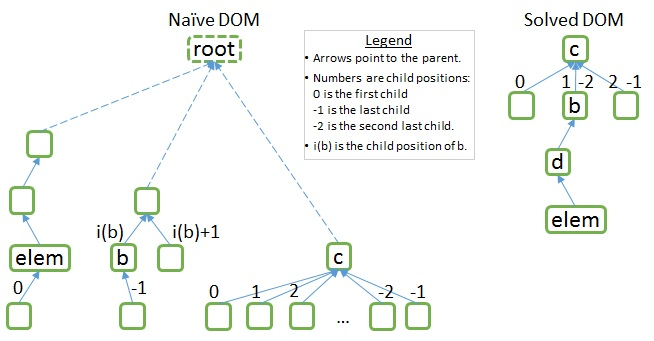
\includegraphics[natwidth=654,natheight=341]{trees.jpg}}}
\caption[Naive vs. Solved DOM trees]{An na\"{i}ve and the solver approach to generating a satisfiable DOM.  The na\"{i}ve DOM attempts and fails to satisfy the DOM operations by simply grouping individual DOM clues and connecting them with a single root (dashed lines).  In the Solved DOM {\tt b} is both child 1 (seocnd child) and child -2 (last child's previous sibling).  {\tt elem} does not have any child because {\tt elem.firstElementChild} is actually in an {\tt or} clause (Sample Code ~\ref{domOr}), in which the solver has decided to make the other sub clause {\tt true}.}
\label{trees}
\end{figure*}


\header{5. 2D Tree Structure \& Implicit Clues.}  
% why quantifiers and not meshing tree pieces together
While many logic solvers natively support single dimensional data types (integers, real numbers and strings), most do not natively support the Document Object Model's 2D tree structure.
A challenge for designing a DOM solver is that the DOM solver must infer indirect or implicit clues before constructing the overall DOM tree.  
For example, when {\tt b.previousElementSibling === c.firstElementChild}, the solver must infer that {\tt c} is the parent of {\tt b}.  

\sloppy{
This type of aliasing can get more complex because DOM operations can be chained.
In JavaScript, a DOM operation on a DOM element (e.g. {\tt elem.parentElement}) returns another DOM element. 
Thus chaining occurs when more DOM operations build on an existing DOM chain.
For example, when we extend the chain {\tt elem.parentElement} with another {\tt .parentElement} DOM operation, {\tt elem.parentElement.parentElement} returns the grandparent of {\tt elem}.
}

\sloppy{
In Sample Code \ref{domOr}, {\tt elem.parentElement.parentElement === c.lastElementChild.previousElementSibling} ({\tt line 12}).
Therefore, the solver has to infer that {\tt b.nextElementSibling} is also {\tt c.lastElementChild} (Figure \ref{trees} Solved DOM), because the code also stated that ({\tt d === b.lastElementChild}) and ({\tt d === elem.parentElement}).  
}

\sloppy{
Once intermediate variables are resolved, the actual length of DOM chains can be observed and chains can span in both parental and sibling dimensions: e.g. {\tt elem.parentElement.parentElement.nextElementSibling}
{\tt .children[2].previousElementSibling}.  
}

A dynamic backward slice can contain multiple long chains.  
Aliasing can become complex because multiple sub-chains of varying length can refer or alias to the same DOM element.  
Thus the DOM tree's 2D structure and implicit clues are another reason for requiring a DOM specific solver.  
A non-solver approach would simply not work when it tries to generate a na\"{i}ve tree (Figure \ref{trees} Na\"{i}ve DOM) by grouping individual DOM chains and connecting them na\"{i}vely to a master root (the dashed lines in Figure \ref{trees}).  


% \header{DOM Mutations}  
% give update score as example
% why conditional slicing
% why 2D is more challenging than 1D
%Expressing the DOM for a solver is not as easy as expressing single dimensional numerical or string operations (e.g. additions and subtractions), because no solver supports 2D tree structures natively and DOM operations are more diverse.  
%Mutations to the DOM tree structure must also be accounted for in both the backward slicing and the solver because changes to the HTML can happen any time during execution.  
%Example mutations include adding or deleting a DOM element (e.g. in the use case of refreshing an email Inbox or deleting a message), or modifying the content or attributes within a DOM element.  
